% !TEX program = xelatex

\documentclass{chicv}
\usepackage{pdfpages}
% optionally suppress printing the page number
\pagenumbering{gobble}

% optional Chinese support
% \useChinese{Medium}{Heavy}
% \useChinese{Regular}{Bold}

\begin{document}

%% basic personal info
\name{Zehao Qian}
\begin{basicinfo}
  \info{\email{zehao.qian.cn@gmail.com}}
  \info{\homepage{GitHub Page}[https://qianzehao123.github.io]}
  \info{\github{QianZehao123}[https://github.com/QianZeHao123]}
  \info{\FreeLeek{FreeLeek \& OpenIE Foundation}[https://github.com/Open-Source-Intelligent-Engineering]}
\end{basicinfo}

\section{Education}
\cventry{Durham University}
  {September 2023 -- July 2024 (Expected)}
  [Master of Science in Data Science (Social Analytics)]
  [Durham, England, British]
\cventry{Zhengzhou University}
  {September 2019 -- July 2023}
  [B.Eng in Industrial Engineering]
  [Zhengzhou, China]
  \begin{itemize}
    \item GPA 82.75/100, Rank 23/102, Scholarship in 2019, 2021, 2022
    \item A+ Courses: Electrotechnics, Contemporary Manufacturing System, Mechanical Manufacturing Engineering, IE software and Application, Enterprise Process Reformation, Engineering Optimization and 16 other programs
    % \item 长中文段落测试:「于是我们奋力前进,却如同逆水行舟,注定要不停地退回过去。」——《了不起的盖茨比》菲茨杰拉德
  \end{itemize}

\section{Honors and Awards}
% \cventry{Mathmatical Modoling}
\begin{compactlist}
  \item \textbf{Computer Algorithms}
    \begin{itemize}
      \item ACM/ICPC - Second Prize of Lanqiao Cup Python Algorithm Competition at Provincial Level
    \end{itemize}
  \item \textbf{Mathematical Modeling}
    \begin{itemize}
      \item The Meritorious Winner Prize of 2023 MCM/ICM - Using Lasso Regression and XGBoost to analyse the relationship between boat size, price and region.
      \item The Second Prize of 2022 12th Mathor Cup College Students Mathematical Contest in Modeling - Solving 5G Base Station Signal Coverage Problems based on Harmony Search Algorithm
    \end{itemize}
  \item \textbf{Innovation and Business Plan Competition}
    \begin{itemize}
      \item First Prize at Provincial Level in Challenge Cup Business Plan Competition (2022) and First Prize at Provincial Level in Challenge Cup First Prize at Provincial Level in Challenge Cup (2023)
      \item First Prize at Provincial Level in E-Commerce Competition Innovation, Creativity and Entrepreneurship (2022)
    \end{itemize}
\end{compactlist}
%
%
\section{Research Experience}
\cventry{Computer and Industrial Engineering Group}
  {September 2021 -- Present}
  % [Server-side Development and Operation and Maintenance Engineer Assistant]
  [Group Member for \textbf{DevOps}, School of Management, Zhengzhou University][\iconlink[\faGithub][CIEG Homepage]{https://ieyjzhou.github.io/lab/}]
    \begin{itemize}
      \item \textbf{Solutions for Tobacco Production (China Tobacco Company Cooperation Project)}
        \begin{itemize}
          \item This project will continue from May 2023 to 2024.
          \item Identification of tobacco pests and diseases and drug dispensing scheme based on Natural language processing and Knowledge graph technology.
          \item Using deep reinforcement learning (pointer network) to optimize cigarette production parameters and improve yield.
        \end{itemize}
      \item \textbf{Teaching Assistant for Engineering Optimization}  \iconlink{https://ieyjzhou.github.io/teaching/}
        \begin{itemize}
          \item In the spring semester of 2023, I made slide and courseware for engineering optimization course, mainly introducing Convex optimization and nonlinear optimization as well as root solution algorithm.
        \end{itemize}
      \item \textbf{A game theory paper -- Web 3D Technologies and Game Theory}
        \begin{itemize}
          \item Constructed supermarket 3D models and customer positioning, used the mapping package called Felt and the Web 3D library Three.js.
          \item Optimized of supermarket collocation based on combinatorial game theory, the paper will be published in journals in Mar.2024.
        \end{itemize}
      \item \textbf{Reinforcement Learning based Q-learning Yard Crane Scheduling Optimization}
        \begin{itemize}
          \item Research on replicating Q-learning algorithm and optimizing container scheduling for yard cranes.
          \item Some mathematical models of the project will be solved using the GJO algorithm, and the relevant research results will be published on IEEE Transaction in Nov 2023.
        \end{itemize}
    \end{itemize}
%
%
%
%
\section{Open-Source Contributions}
%
%
\cventry{Nashsweeper}
  {Dec 2022 -- May 2023}
  [Project Author (Excellent Graduation Thesis)]
  [\iconlink[\faGithub][Nashsweeper Repo]{https://github.com/QianZeHao123/Nashsweeper}]
  \begin{itemize}
    \item Nashsweeper shows a playful introduction of Nash equilibrium and designs a game named Nashsweeper, which is a game designed to find the pure strategy. \iconlink[\faGlobe][iPad Version]{http://74.48.4.203:8080/} \iconlink[\faGlobe][PC Version]{http://74.48.4.203:8080/}
    \item Nashsweeper core computing engine adopts the reget-value algorithm implemented with SQLite. As a Python package, it can be invoked in jupyter- notebook to deal with industrial and data science problems.
  \end{itemize}
%
%
%
\cventry{OpenIE -- Open Source Industrial Engineering Foundation}
  {April 2022 -- Present}
  [Foundation Initiator, Project Leader]
  [\iconlink[\faGlobe][OpenIE foundation]{https://qianzehao123.github.io/OpenIE/}]
  \begin{itemize}
    \item Prediction of Tool Wear in Machining Centers Based on Deep Learning and Its Industrial Application (Feature engineering and Recurrent neural network are used in this project). \iconlink[\faGlobe][OpenIE Repo]{https://github.com/Open-Source-Intelligent-Engineering/OpenIE-WaveAnalysis}
    \item Some other optimizations for industrial scenario problems.
  \end{itemize}
%
%
\cventry{FreeLeek}
  {Oct 2021 -- Present}
  [Project Author and Maintainer]
  [\iconlink[\faGithub][FreeLeek]{https://gitee.com/qian_zehao/free-leek} \iconlink[\faGithub][FreeLeek-ESP32]{https://gitee.com/qian_zehao/leek-box}]
  \begin{itemize}
    \item FreeLeek is an open source server-end framework for transmiting financial data to app backend and WeChat platform by using Python Flask, Tushare Pro and Akshare.
    \item FreeLeek can automatically push finance news to WeChat official account subscribed by user.
    \item More users' function can be defined easily by editing python script such as quant trade algorithms, stock position management system.
  \end{itemize}
%
%
%
\section{Internship Experience}
%
%
\cventry{Tianjin Jinmao Int'l Freight Co., Ltd}
  {Jan 2022 -- Feb.2022, Jun 2022 -- Sep.2022}
  [Server-side Development and Operation and Maintenance Engineer Assistant][Tianjin, China]
  \begin{itemize}
    \item Engaged in server operation and maintenance, back-end development, and database management. 
    \item Developed company's enterprise resource planning system (ERP) and customer management system (CMS) utilizing JavaScript and MySQL, contributing to the company's enterprise digitalization.
  \end{itemize}
%
%
\section{Skills}

\begin{compactlist}
  % \item \textbf{English Evidence}: IELTS 6.5 with every element above 6.0 (23/06/2023)
  \item \textbf{Full Stack Programming}: Python (Flask framework for Backend Dev and a little PyTorch), Node.js (Vue framework for Frontend Dev) and MatLab (for Machine Learning and Signal Processing)
  \item \textbf{Computer Skills}: Docker Deployment, Unity, Simulation Software, Statistic and Optimization, FlexSim(for logistics), LaTeX (I used it to edit this CV) and SPSS.
  \item \textbf{Hands-on ability and musical talent}: Mechanical modeling, 3D printing and Hardware making. Proficient in guitar, bass, piano, and other musical instruments.

\end{compactlist}
%
%
% 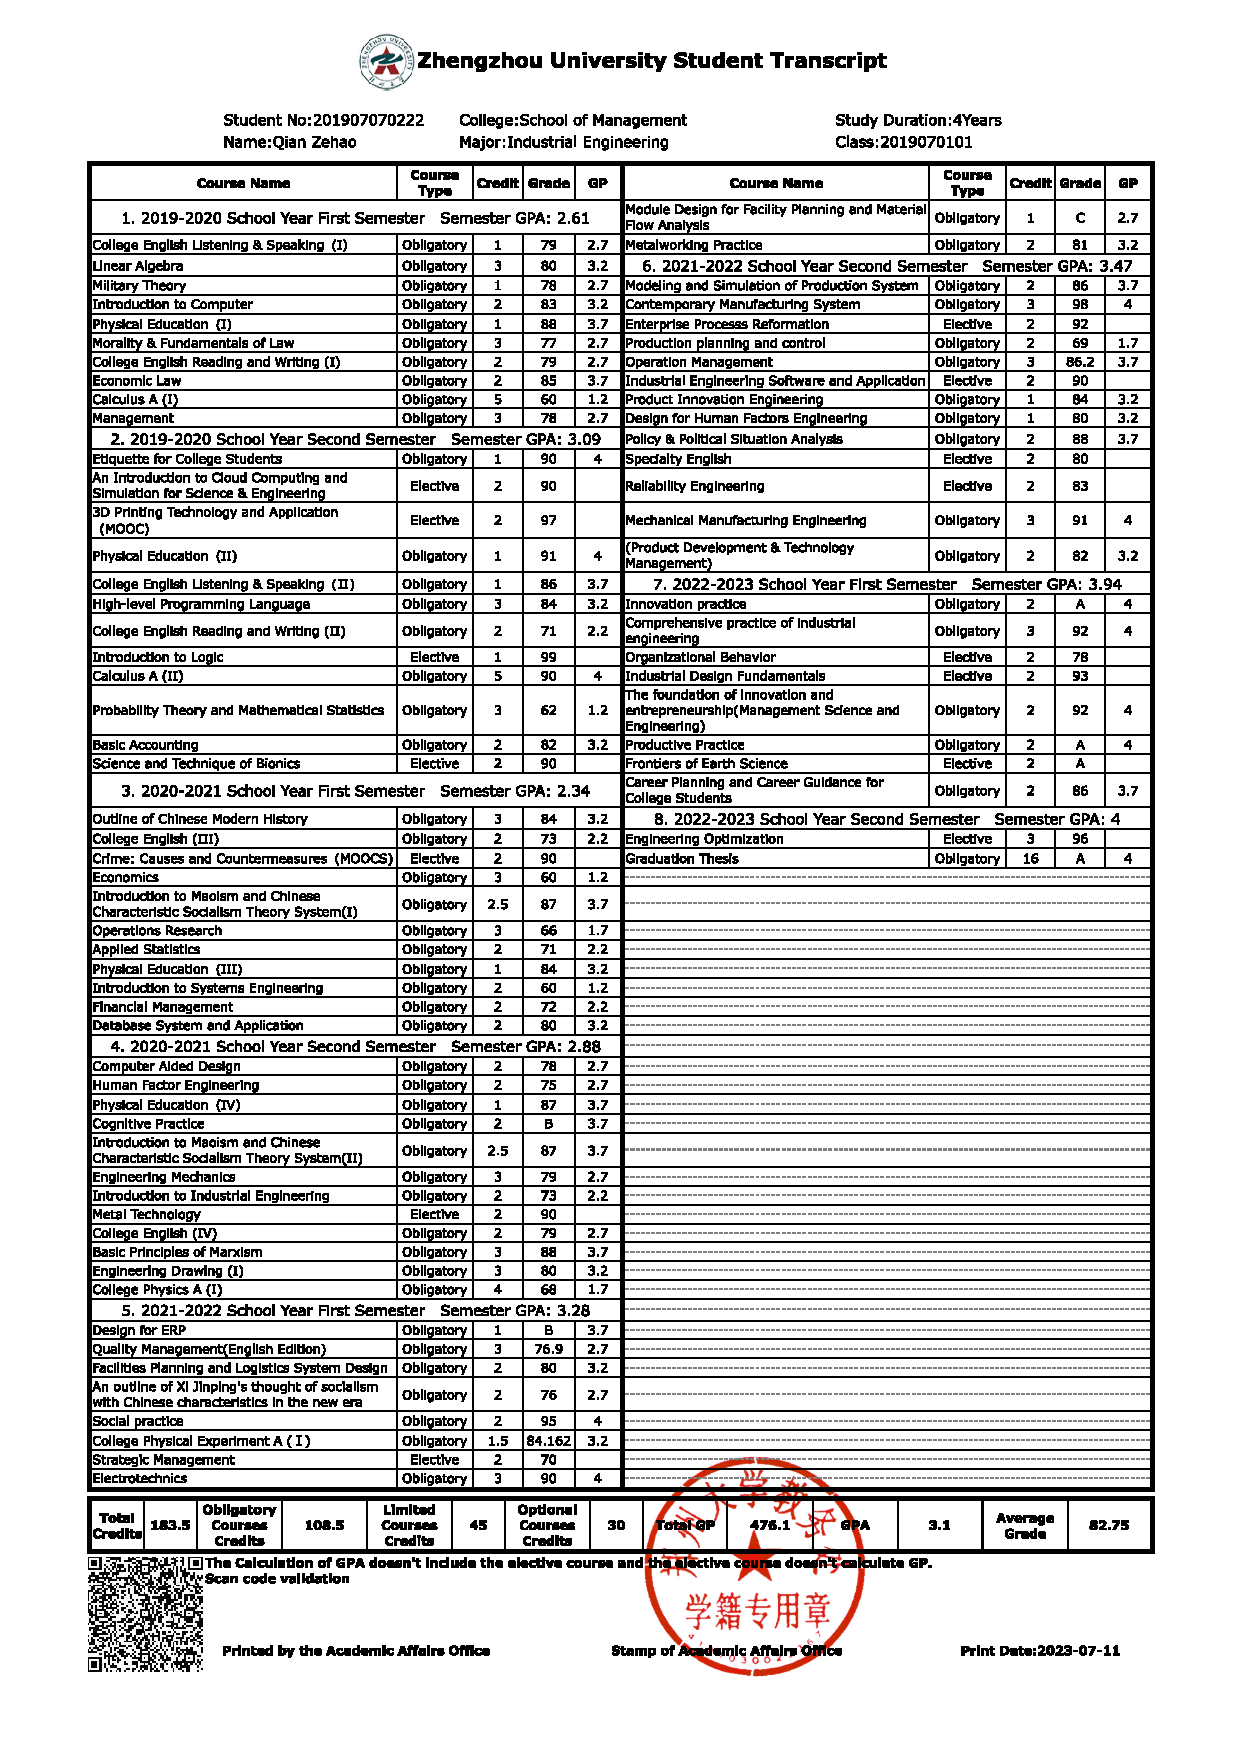
\includepdf[pages={1}]{img/Transcript.pdf}
%
%
\end{document}
